%====================================================================
%====================================================================
\section{Variational inference for the stochastic block model}
\subsection*{Model}
\frame{\frametitle{Outline} \tableofcontents}
\frame{\frametitle{Outline} \tableofcontents[currentsection]}
%====================================================================
\frame{\frametitle{Binary SBM} 

  \paragraph{Data at hand.}
  \begin{itemize}
   \item $Y = (Y_{ij})_{1 \leq i, j, \leq n}= n \times n$ matrix: 
   $$
   Y_{ij} =  \text{link between individual $i$ and $j$}
   $$
  \end{itemize}
  
  \bigskip \pause
  \paragraph{Model.} $K$ groups
  \begin{itemize}
  \item $(Z_i)_{1 \leq i \leq n} = $ iid node memberships (with proportion $\pi$)
  \item $(Y_{ij})_{1 \leq i, j \leq n} =$ conditionally independant : $P(Y_{ij} = 1 \mid Z_i, Z_j ) = p_{k\ell}$
  \end{itemize}

  $$
  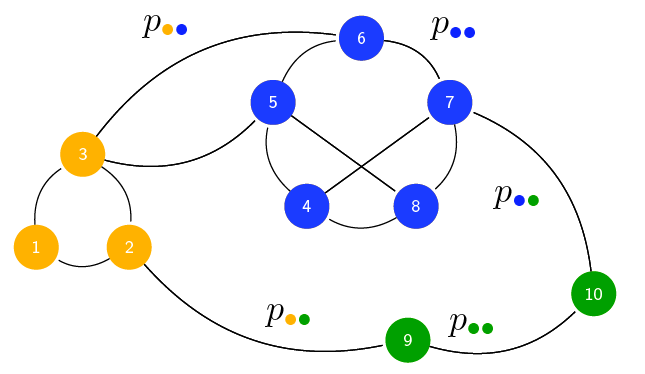
\includegraphics[width=.4\textwidth]{../FIGURES/SBM-CMatias}
  $$
}

%====================================================================
\frame{\frametitle{General SBM} 

  \paragraph{Data at hand.}
  \begin{itemize}
   \item $Y = (Y_{ij})_{1 \leq i, j, \leq n}= n \times n$ matrix: 
   $$
   Y_{ij} =  \text{interaction strength between individual $i$ and $j$}
   $$
   \item $x_{ij} =$ vector of covariates\footnote{In many applications, clustering nodes without accounting for known effects is often useless} for the pair $(i, j)$
  \end{itemize}
  
  \bigskip \bigskip \pause
  \paragraph{Model.} $K$ groups
  \begin{itemize}
  \item Same $(Z_i)$ as before
  \item $(Y_{ij})_{1 \leq i, j \leq n} =$ conditionally independant : $Y_{ij} \mid Z_i, Z_j \sim f(\cdot; \gamma_{Z_i Z_j}, x_{ij}) $
  \end{itemize}

  \bigskip \bigskip \pause
  \paragraph{Example.} GLM framework:
  \begin{align*}
  \log f(Y_{ij}; \gamma_{kl}, x_{ij}) & = (\eta_{ij}^{k\ell})^\intercal t(Y_{ij}) - a(Y_{ij}) - b(\eta_{ij}^{k\ell}) \\
  \eta_{ij}^{k\ell} & = \alpha_{kl} + \emphase{x_{ij}^\intercal \beta}
, 
  \qquad \gamma_{kl} = (\alpha_{kl}, \beta), 
  \quad \theta = (\pi, \alpha, \beta)
  \end{align*}
}

%====================================================================
\subsection*{Inference}
%====================================================================
\frame{\frametitle{Inference} 

  \paragraph{Maximum likelihood inference via EM:} requires to evaluate $p(Z \mid Y)$
  
  \bigskip \bigskip 
  \begin{overprint}
  \onslide<1> \paragraph{Graphical model point of view.} $p(Z)$
  \onslide<2> \paragraph{Graphical model point of view.} $p(Z) p(Y \mid Z)$
  \onslide<3> \paragraph{Graphical model point of view.} Moralization
  \onslide<4> \paragraph{Graphical model point of view.} $p(Z \mid Y)$
  \end{overprint}
  ~\\ ~\
    
  \begin{overprint}
  \onslide<1>
  \begin{centering}
    \begin{tikzpicture}
  \node[hidden] (Z1) at (0, \edgeunit) {$Z_1$};
  \node[hidden] (Z2) at (\edgeunit, \edgeunit) {$Z_2$};
  \node[hidden] (Z3) at (0, 0) {$Z_3$};
  \node[hidden] (Z4) at (\edgeunit, 0) {$Z_4$};

  \node[empty] (Y12) at (.5*\edgeunit, 1.75*\edgeunit) {$Y_{12}$};
  \node[empty] (Y13) at (-.75*\edgeunit, .5*\edgeunit) {$Y_{13}$};
  \node[empty] (Y14) at (1.75*\edgeunit, 1.75*\edgeunit) {$Y_{14}$};
  \node[empty] (Y23) at (-.75*\edgeunit, 1.75*\edgeunit) {$Y_{23}$};
  \node[empty] (Y24) at (1.75*\edgeunit, .5*\edgeunit) {$Y_{24}$};
  \node[empty] (Y34) at (.5*\edgeunit, -.75*\edgeunit) {$Y_{34}$};
  
%   \draw[arrow] (Z1) to (Y12);  \draw[arrow] (Z2) to (Y12);
%   \draw[arrow] (Z1) to (Y13);  \draw[arrow] (Z3) to (Y13);
%   \draw[arrow] (Z1) to (Y14);  \draw[arrow] (Z4) to (Y14);
%   \draw[arrow] (Z2) to (Y23);  \draw[arrow] (Z3) to (Y23);
%   \draw[arrow] (Z2) to (Y24);  \draw[arrow] (Z4) to (Y24);
%   \draw[arrow] (Z3) to (Y34);  \draw[arrow] (Z4) to (Y34);
  \end{tikzpicture}

 
  \end{centering}
  \onslide<2>
  \begin{centering}
    \begin{tikzpicture}
  \node[hidden] (Z1) at (0, \edgeunit) {$Z_1$};
  \node[hidden] (Z2) at (\edgeunit, \edgeunit) {$Z_2$};
  \node[hidden] (Z3) at (0, 0) {$Z_3$};
  \node[hidden] (Z4) at (\edgeunit, 0) {$Z_4$};

  \node[observed] (Y12) at (.5*\edgeunit, 1.75*\edgeunit) {$Y_{12}$};
  \node[observed] (Y13) at (-.75*\edgeunit, .5*\edgeunit) {$Y_{13}$};
  \node[observed] (Y14) at (1.75*\edgeunit, 1.75*\edgeunit) {$Y_{14}$};
  \node[observed] (Y23) at (-.75*\edgeunit, 1.75*\edgeunit) {$Y_{23}$};
  \node[observed] (Y24) at (1.75*\edgeunit, .5*\edgeunit) {$Y_{24}$};
  \node[observed] (Y34) at (.5*\edgeunit, -.75*\edgeunit) {$Y_{34}$};
  
  \draw[arrow] (Z1) to (Y12);  \draw[arrow] (Z2) to (Y12);
  \draw[arrow] (Z1) to (Y13);  \draw[arrow] (Z3) to (Y13);
  \draw[arrow] (Z1) to (Y14);  \draw[arrow] (Z4) to (Y14);
  \draw[arrow] (Z2) to (Y23);  \draw[arrow] (Z3) to (Y23);
  \draw[arrow] (Z2) to (Y24);  \draw[arrow] (Z4) to (Y24);
  \draw[arrow] (Z3) to (Y34);  \draw[arrow] (Z4) to (Y34);
  \end{tikzpicture}

 
  \end{centering}
  \onslide<3>
  \begin{centering}
    \begin{tikzpicture}
  \node[hidden] (Z1) at (0, \edgeunit) {$Z_1$};
  \node[hidden] (Z2) at (\edgeunit, \edgeunit) {$Z_2$};
  \node[hidden] (Z3) at (0, 0) {$Z_3$};
  \node[hidden] (Z4) at (\edgeunit, 0) {$Z_4$};

  \node[observed] (Y12) at (.5*\edgeunit, 1.75*\edgeunit) {$Y_{12}$};
  \node[observed] (Y13) at (-.75*\edgeunit, .5*\edgeunit) {$Y_{13}$};
  \node[observed] (Y14) at (1.75*\edgeunit, 1.75*\edgeunit) {$Y_{14}$};
  \node[observed] (Y23) at (-.75*\edgeunit, 1.75*\edgeunit) {$Y_{23}$};
  \node[observed] (Y24) at (1.75*\edgeunit, .5*\edgeunit) {$Y_{24}$};
  \node[observed] (Y34) at (.5*\edgeunit, -.75*\edgeunit) {$Y_{34}$};
  
  \draw[lightarrow] (Z1) to (Y12);  \draw[lightarrow] (Z2) to (Y12);
  \draw[lightarrow] (Z1) to (Y13);  \draw[lightarrow] (Z3) to (Y13);
  \draw[lightarrow] (Z1) to (Y14);  \draw[lightarrow] (Z4) to (Y14);
  \draw[lightarrow] (Z2) to (Y23);  \draw[lightarrow] (Z3) to (Y23);
  \draw[lightarrow] (Z2) to (Y24);  \draw[lightarrow] (Z4) to (Y24);
  \draw[lightarrow] (Z3) to (Y34);  \draw[lightarrow] (Z4) to (Y34);
  
  \draw[dashededge] (Z1) to (Z2);  \draw[dashededge] (Z1) to (Z3);
  \draw[dashededge] (Z1) to (Z4);  \draw[dashededge] (Z2) to (Z3);
  \draw[dashededge] (Z2) to (Z4);  \draw[dashededge] (Z3) to (Z4);
  \end{tikzpicture}

 
  \end{centering}
  \onslide<4>
  \begin{centering}
    \begin{tikzpicture}
  \node[hidden] (Z1) at (0, \edgeunit) {$Z_1$};
  \node[hidden] (Z2) at (\edgeunit, \edgeunit) {$Z_2$};
  \node[hidden] (Z3) at (0, 0) {$Z_3$};
  \node[hidden] (Z4) at (\edgeunit, 0) {$Z_4$};

  \node[eliminated] (Y12) at (.5*\edgeunit, 1.75*\edgeunit) {$Y_{12}$};
  \node[eliminated] (Y13) at (-.75*\edgeunit, .5*\edgeunit) {$Y_{13}$};
  \node[eliminated] (Y14) at (1.75*\edgeunit, 1.75*\edgeunit) {$Y_{14}$};
  \node[eliminated] (Y23) at (-.75*\edgeunit, 1.75*\edgeunit) {$Y_{23}$};
  \node[eliminated] (Y24) at (1.75*\edgeunit, .5*\edgeunit) {$Y_{24}$};
  \node[eliminated] (Y34) at (.5*\edgeunit, -.75*\edgeunit) {$Y_{34}$};
  
  \draw[edge] (Z1) to (Z2);  \draw[edge] (Z1) to (Z3);
  \draw[edge] (Z1) to (Z4);  \draw[edge] (Z2) to (Z3);
  \draw[edge] (Z2) to (Z4);  \draw[edge] (Z3) to (Z4);
  \end{tikzpicture}

 
  \end{centering}
  \end{overprint}

}

%====================================================================
\frame{\frametitle{Variational inference} 

  \paragraph{Variational approximation.} Choose
  \begin{itemize}
   \item a divergence measure $D(q \mid\mid p)$
   \item a class of distributions $\Qcal$
  \end{itemize}
  and maximize wrt $\theta$ and $q \in \Qcal$ the lower bound \refer{WaJ08,BKM17}
  $$
  \log p_\theta(Y) - D(q(Z) \mid\mid p_\theta(Z \mid Y)) \leq \log p_\theta(Y)
  $$

  \bigskip \bigskip \pause
  \paragraph{Popular choice for SBMs \refer{DPR08,Leg16,MaM16}.} $D = KL$ so
  \begin{align*}
    J(\theta, q) 
    & := \log p_\theta(Y) - KL(q(Z) \mid\mid p_\theta(Z \mid Y)) \\
    & = \Esp_q \left( \log p_\theta(Y, Z) \right) - \Esp_q\left( q(Z) \right)
  \end{align*}
  and $q$ factorizable: 
  $
  \Qcal = \left\{q(Z): q(Z) = \prod_i q_i(Z_i)\right\}.
  $
  
}

%====================================================================
\frame{\frametitle{Extensions and properties} 

  \paragraph{Variational Bayes (VBEM).} Variational approximations can be designed in a Bayesian framework \refer{LBA12,LaR16} to get
  $$
  q(\theta, Z) \approx p(\theta, Z \mid Y), 
  \qquad q \in \Qcal
  $$
  \ra Easier with conjugate priors.

  \bigskip \bigskip \pause
  \paragraph{Practical advantages:} 
  \begin{itemize}
   \item Easy to implement
   \item Converges reasonably fast, 
   \item Works well in practice (simulations)
  \end{itemize}
 

  \bigskip \bigskip \pause
  \paragraph{Theoretical guaranties.} Very few
  \begin{itemize}
   \item except in the binary case, without covariates \refer{CDP12,BCC13,MaM15}
  \end{itemize}

}


